\section{Details on Experiments with Human Participants}
\label{app:human_exp_details}
\begin{figure}[t!]
    \begin{center}
        \begin{small}
            \begin{center}
                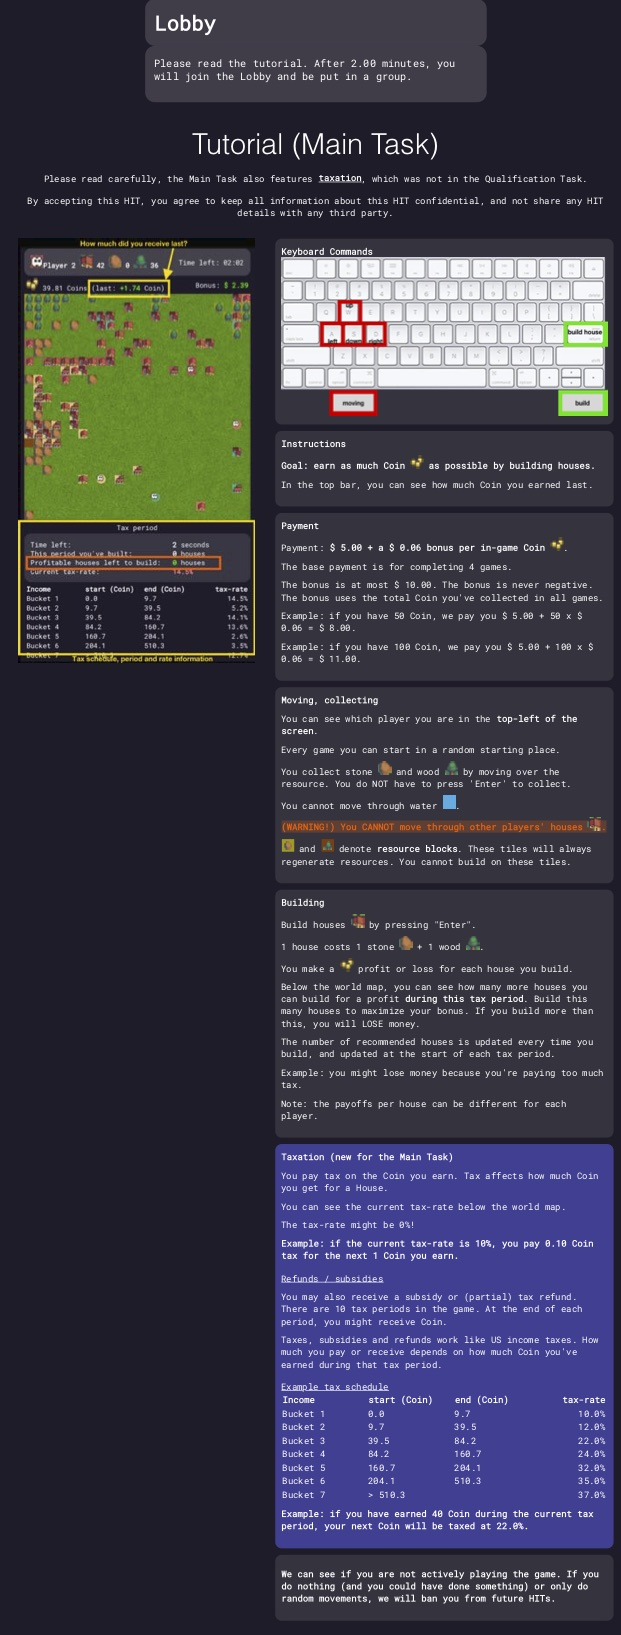
\includegraphics[width=0.4\linewidth]{figures/human_gui_tutorial.jpg}
            \end{center}
            \caption{The starting point for each experiment was the lobby and tutorial (Figure \ref{fig:human_exp_gui_tutorial}). The tutorial explained all rules of the world and the objective for each participant. It also explained how the variable part of payment for the experiment was computed. In addition, an example of the graphical interface and keyboard controls was shown. Participants were warned not to idle in the game. Participants were given 2 minutes before the start of the experiment to read the tutorial. After this initial period, as soon as there were enough participants to form a group, the lobby system presented the participants in the new group with the experiment's main page.}
            \label{fig:human_exp_gui_tutorial}
        \end{small}
    \end{center}
\end{figure}
\begin{figure}[t!]
    \begin{center}
        \begin{small}
            \begin{center}
                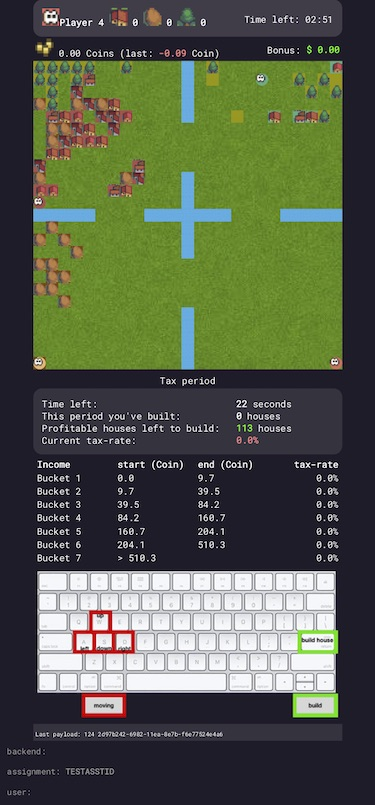
\includegraphics[width=0.5\linewidth]{figures/human_gui_main.jpg}
            \end{center}
            \caption{The main experiment's graphical user interface (Figure \ref{fig:human_exp_gui_main}) showed (from top to bottom): the endowment of the agent, the remaining time in the episode, the bonus amount earned so far, the spatial state of the world, the tax information and current tax rate, the time left, the number of houses built and the number of profitable houses left to build. Below all data, a reminder of the controls was shown as well. After an episode was over, participants were returned to the lobby (if the participant had seen less than 4 episodes) or survey (if 4 episodes had been seen).
            }
            \label{fig:human_exp_gui_main}
        \end{small}
    \end{center}
\end{figure}
\begin{figure}[t!]
    \begin{center}
        \begin{small}
            \begin{center}
                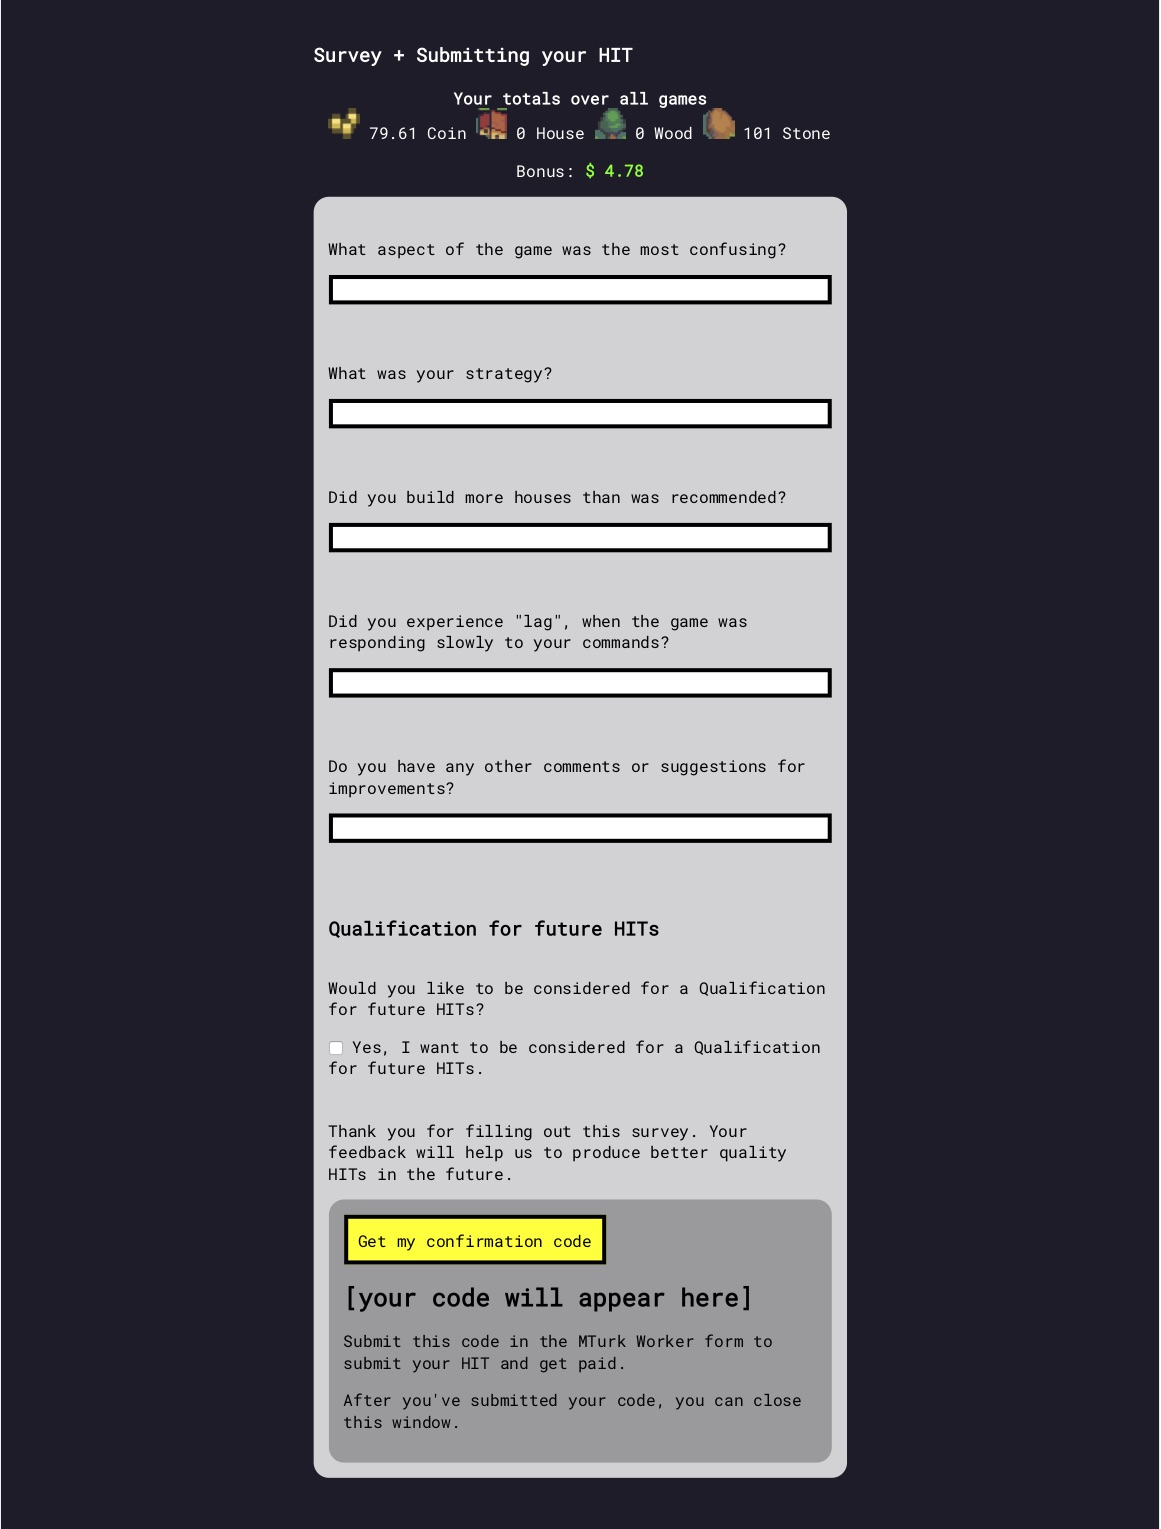
\includegraphics[width=0.8\linewidth]{figures/human_gui_survey.jpg}
            \end{center}
            \caption{The post-experiment survey showed how much the participant had collected in terms of resources, coin and bonus. It also asked questions about the participants experience, strategy and general feedback on the experiment. For instance, participants could communicate technical issues, such as lag. At the end of the survey, participants were given a confirmation code that allowed them to confirm successful completion of the task on the Amazon Mechanical Turk platform.}
            \label{fig:human_exp_gui_survey}
        \end{small}
    \end{center}
\end{figure}

All experiment modules used with human participants are shown and described in Figures \ref{fig:human_exp_gui_tutorial} (lobby, tutorial), \ref{fig:human_exp_gui_main} (main graphical interface), and \ref{fig:human_exp_gui_survey} (survey).

